
\chapter{My Proposal}
\label{chapt:proposal}


As section~\ref{setc:ChallengesData} demonstrates, the Megason lab's datasets are hard to proceed. That forces us to find innovative solution for problems that may seem simple at first glance.

This chapter describes the new method we proposed in order to solve the nuclei detection problem. This new method uses a different approaches based on the membrane information as principal and not complimentary information. We shall first introduce the theorical concepts of this method, and prove its functioning on a simple dataset.


All the papers we have been reading take advantage of the nuclei channel information, but none of them takes advantage of the membrane channel.
This channel provides capital information, especially in the case of stuck nuclei, where most common detection method fail.
Indeed, the membrane can separate the different nuclei.
We propose here a method using the membrane information in an original way.



%%%%%%%%%%%%%%%%%%%%%%%%%%%%%%%%%%%%%%%%%%%%%%%%%%%%%%%%%%%%%%%%%%%%%%%%%%%%%%%
%%%%%%%%%%%%%%%%%%%%%%%%%%%%%%%%%%%%%%%%%%%%%%%%%%%%%%%%%%%%%%%%%%%%%%%%%%%%%%%
%%%%%%%%%%%%%%%%%%%%%%%%%%%%%%%%%%%%%%%%%%%%%%%%%%%%%%%%%%%%%%%%%%%%%%%%%%%%%%%


\section{Preliminaries}
\label{sect:definitions}
We present here the mathematical concepts used by the proposal.


\subsection{Euclidean distance map}
\label{subsec:EuclDistMapDef}
Let \( I : \Omega \subset \mathbb{Z}^3 \leftarrow \{0,1\} \) be a binary image where the domain \({\Omega}\) is convex, in particular, \( \Omega  = \{1,{\dots},n\}{\times}\{1,{\dots},n\}{\times}\{1,{\dots},n\} \). By convention, 0 is associated to black and 1 to white, Hence we have an object \({\mathcal{O}}\) represented by all the white pixels:\\
\begin{center}
\( {\mathcal{O}} = p \in \Omega \mid I(p)=1 \)
\end{center}

The set \({\mathcal{O}}\) is called object or foreground and can consist of any subset of the image domain, including disjoint sets.
The elements of its complement,\(\overline{\mathcal{O}}\), the set of black pixels in \({\Omega}\), are called background.
\begin{itemize}
\item For two pixels, \({p : (p_x, p_y, p_z)}\) , and \({q : (q_x, q_y, q_z)}\), the Euclidean distance is given by : 
\[
d(p,q) = \sqrt{ (p_x-q_x)^{2}+(p_y-q_y)^{2}+(p_z-q_z)^{2} }
\]
%
\item The distance transform (DT) is the transformation that generates a map \({D}\) whose value in each pixel \({p}\) is the smallest distance from this pixel to \(\overline{\mathcal{O}}\):
\[
D(p) := min\{ d(p,q) \mid q \in \overline{\mathcal{O}}\} = min\{ d(p,q) \mid I(q) = 0 \}
\]
The image \({D}\) is called the distance map of \({I}\).
\end{itemize}


\subsection{Voronoi diagram}

We define here the \emph{point-wise Voronoi diagram} (VD) and related concepts.
The \emph{Voronoi region} (VR) of an interest point is the set of points strictly closer to it than to any other interest point. The \emph{Voronoi element} closest to a given pixel \({p}\) is denoted by {\( VS(p) \)}. In case \({p}\) has two or more closest \emph{sites}, one of them is arbitrarily chosen to be {\( VS(p) \)}. By definition, the point-wise Voronoi diagram is the set of points closest to one or more \emph{sites}, that is, the points not in any Voronoi region. A Voronoi partition is the collection of the VRs of all \emph{sites} or \emph{seeds}. To build the partition, each point of the VD is arbitrarily attributed to the VR of one of the \emph{sites} minimally equidistant to it.
The Voronoi partition can be represented by the label map, where each VS has an associated label (a number) that identifies this VS and pixels of its VR. The label map is formally defined as:

\[
Label : \Omega \rightarrow \{ 1,{\dots},n_s \}  \\
p \rightarrow Label(p) = \{ Label(q) \mid q = VS(p) \}
\]
where \({n_s}\) is the number of \emph{sites} (and of VRs).

%\xmapsto


\subsection{Centroid}

The \emph{centroid} \({c_\mathcal{O}}\) of an object \({\mathcal{O}}\) is defined as:
\[
c_O :=  \sum_{p \in {O}} \frac{p}{Card(O)}
\]


\subsection{Assumptions}

\begin{figure}[h]
\begin{center}
\leavevmode
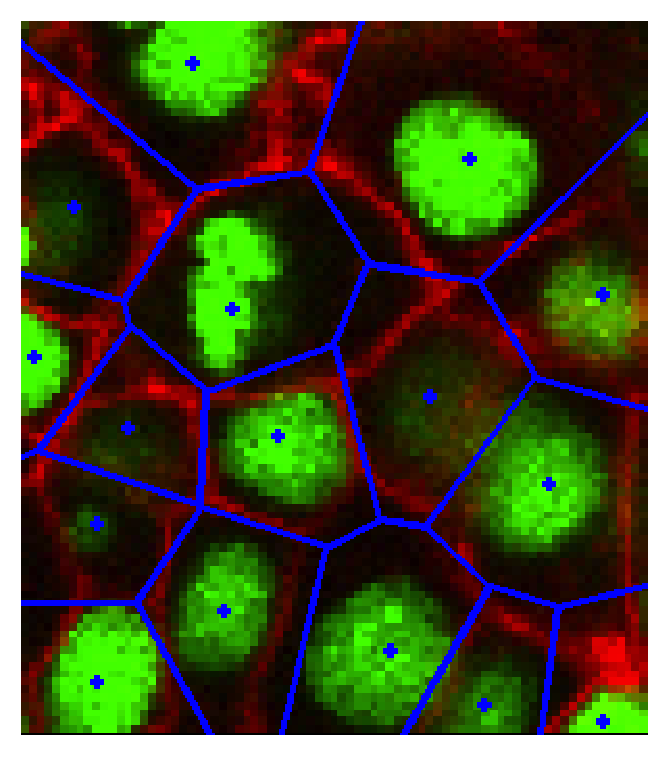
\includegraphics[width=0.5\textwidth]{pictures/voronoiExample2D}
\end{center}
\caption{Boundary of Voronoi regions (blue) generated from each cell nuclei (green), with the membrane (red). The Voronoi  diagram was generated in 2D.}
\label{fig:voronoiExample2D}
\end{figure}

\begin{figure}[h]
\begin{center}
\leavevmode
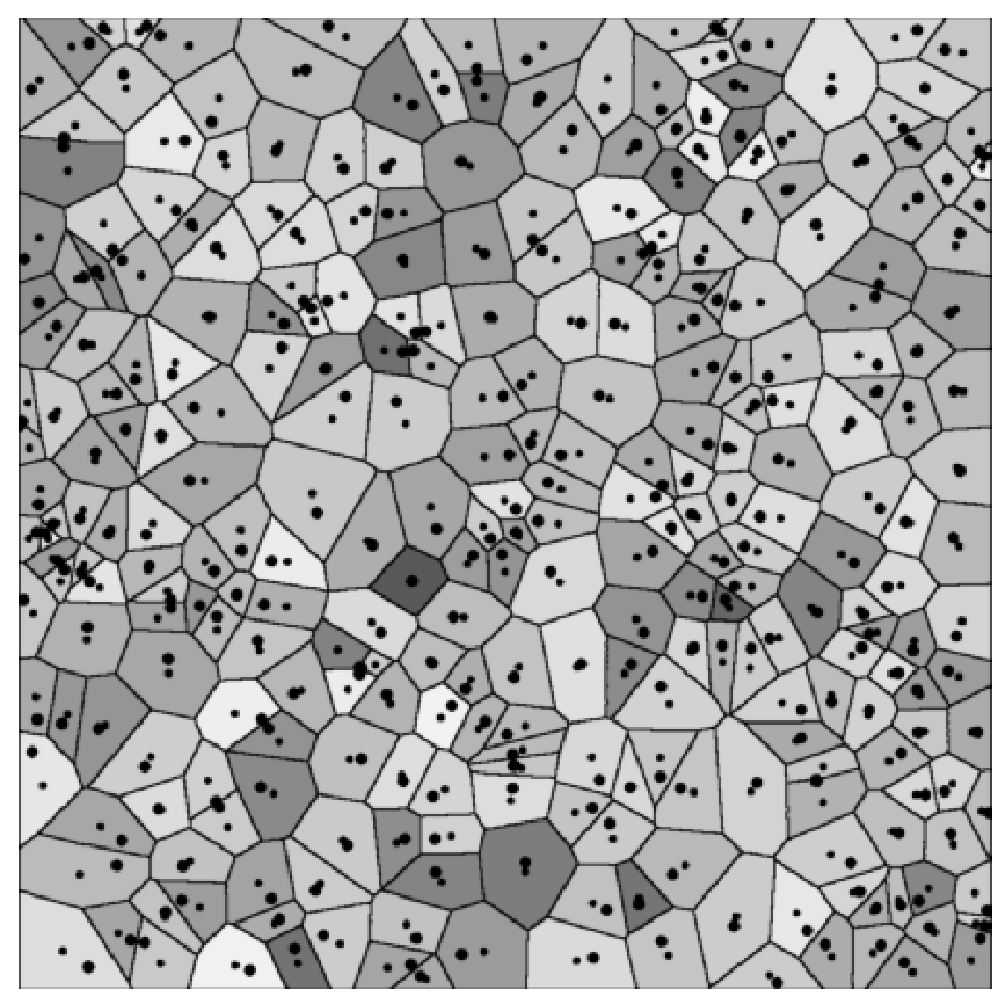
\includegraphics[width=0.5\textwidth]{pictures/centroidVoronoi}
\end{center}
\caption{Voronoi diagram with \emph{sites} (large dots) and centroids (small dots). Image from~\cite{Secord02randommarks}.}
\label{fig:centroidVoronoi}
\end{figure}


Several article make use of \emph{Voronoi diagrams} to model the membrane of cells~\cite{luengo2008can,yu2010evolving}.
But the membrane is also around each nuclei. So the membrane channel provides us with information about nuclei positions.
We based our algorithm on two assumptions :
\begin{itemize}
\item The membrane can be considered as a \emph{Voronoi diagram}.
\item Nuclei are in the center of cells, and correspond to the \emph{sites} of the \emph{Voronoi diagram}.
\end{itemize}
We can see figure~\ref{fig:voronoiExample2D}, that the membrane can be approximated by a \emph{Voronoi diagram} centred in each nucleus.
From this, we can use the membrane channel and consider it as a \emph{Voronoi tessellation}.


%%%%%%%%%%%%%%%%%%%%%%%%%%%%%%%%%%%%%%%%%%%%%%%%%%%%%%%%%%%%%%%%%%%%%%%%%%%%%%%
%%%%%%%%%%%%%%%%%%%%%%%%%%%%%%%%%%%%%%%%%%%%%%%%%%%%%%%%%%%%%%%%%%%%%%%%%%%%%%%
%%%%%%%%%%%%%%%%%%%%%%%%%%%%%%%%%%%%%%%%%%%%%%%%%%%%%%%%%%%%%%%%%%%%%%%%%%%%%%%


\section{Method}

\begin{figure}[h]
\begin{center}
\leavevmode
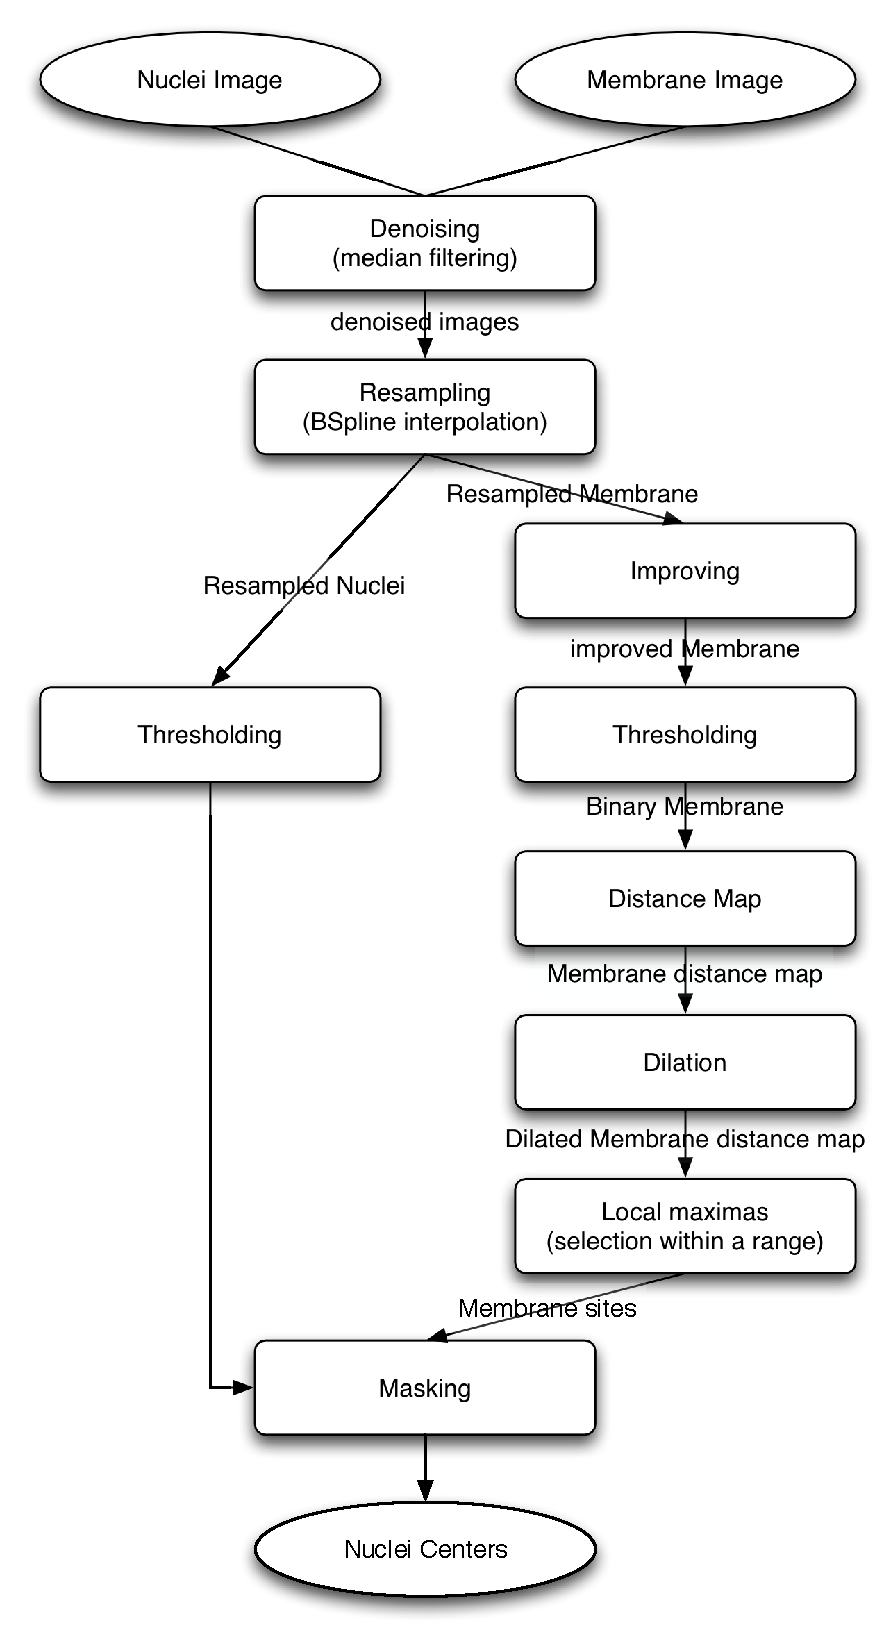
\includegraphics[height=0.87\textheight]{pictures/proposalFlowchart}
\end{center}
\caption{Flowchart of the proposed algorithm.}
\label{fig:propFlowchart}
\end{figure}

As defined in \ref{sect:definitions},the \emph{Voronoi cells} (or VRs) are constituted by all the points closer to the \emph{site} of the cell than any other \emph{site}.

We have a damaged information about the boundaries of the VRs. In order to reconstruct a \emph{Voronoi diagram},
 we consider that the cell membrane represents a \emph{centroidal Voronoi tessellation} (see figure~\ref{fig:centroidVoronoi}): we locate the centroid of each VR, and from that, estimate the position of the nuclei.
 
We use the distance map information to find a subset of the VR within the damaged membrane cells.
Using this distance information, we find an approximation of the VR (approximate VR), and we use the centroid of this region to approximate the location of the \emph{site}.
We will first describe our algorithm. We will then introduce the difficulties we encountered (see section~\ref{sect:difficultiesTheory}), and prove that even with noisy and incomplete membrane information, we are able to find the approximate position of the \emph{sites}.


\subsection{Algorithm pipeline}

It is clear that for most image processing problems, a series of transformation is needed in order to be able to work with the data.
Inspired by the described articles, I designed an image processing pipeline adapted to our data.
I describe here the image processing pipeline for the new algorithm, and the improvements of the existing nuclei segmentation pipeline
\begin{description}
  \item[Denoising: ] We first process the membrane and the nuclei channel with a median filter. The median filter's structuring element is a disk of radius one third of the radius of a nuclei, for the nuclei channel, and one third of the thickness of the membrane for the membrane channel.
  We process the images before resampling, as the resampling on the z stack spreads noisy points, invalidating the median filter's use.
%
%
  \item[Images Resampling: ] As in~\cite{li20073}, our images are anisotropic : they are very high resolution in xy, and very low resolution in z, as shown by the
  table~\ref{tab:DataSizes}, and the figure~\ref{fig:anisotropy}.
  We don't need this much information in xy, as algorithms are computationally expensive, and we want to keep a reasonable processing time.
  But, we need a higher resolution in z.
  For that purpose, we resample our images, using a BSpline interpolation of order 5.
  This technique provides us with an isotropic dataset of spacing 0.4um, that can easily be
  processed by the other filters. The interpolation, in the z direction, partially reconstructs the membrane.
%
%
  \item[Nuclei binary mask: ] We threshold the nuclei image to keep a rough binary mask in which the nuclei are present (see figure~\ref{fig:propNucleiMask}).
  The thresholds are chosen empirically after an analysis of the histogram of the nuclei images.
%  
%
%  
  \item[Distance map creation: ] We then process the resampled and denoised membrane channel with Kishore's membrane reconstruction filter.
  The resultant membrane is thresholded to get a binary image from which we compute a distance map (see figure~\ref{fig:propDistance})
  using the algorithm proposed by Maurer Jr {\etal}~\cite{maurer2003linear}, as it is the fastest for big binary images with complex structures according to~\cite{distanceMapReview}.
  The threshold values are empirically determined.
%  
%
%
  \item[Approximate Voronoi Cell extraction: ] Then, we threshold the distance map with a threshold value of one third of a nuclei radius.
  From this thresholding, we get a set of regions located inside each cell : the approximate VRs (see figure~\ref{fig:propThresholdedDistanceMap}).
  If the assumption that holes are much smaller than nuclei radius is correct, those regions should not touch because the distance map should not have high value between different VRs. We use a labelling procedure, to separate each of these regions.
%
%
  \item[Nuclei detection: ] We finally locate the centroid of each approximate VR and output this result as cell nuclei detection.
%  
%
%
\end{description}


\begin{figure}[h]
  \centering
\subfloat[][]{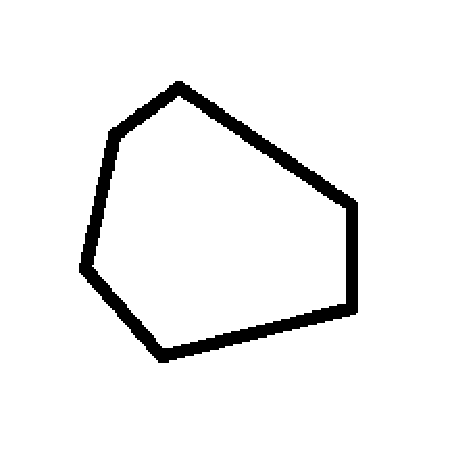
\includegraphics[width=0.33\textwidth, height=0.33\textwidth]{pictures/theoryComplete}\label{fig:theoryComplete}}
\subfloat[][]{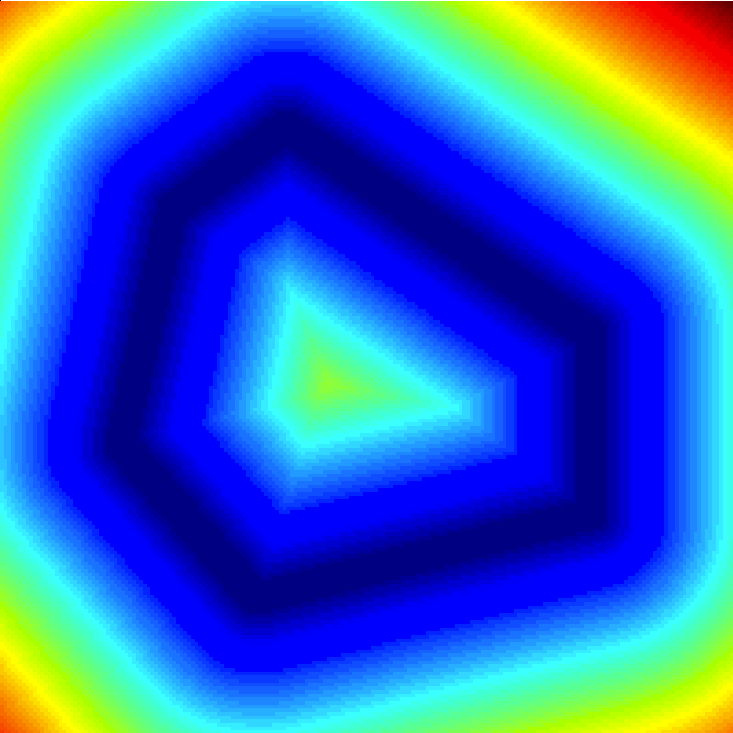
\includegraphics[width=0.33\textwidth, height=0.33\textwidth]{pictures/theoryCompleteDistance}\label{fig:theoryCompleteDistance}}
\subfloat[][]{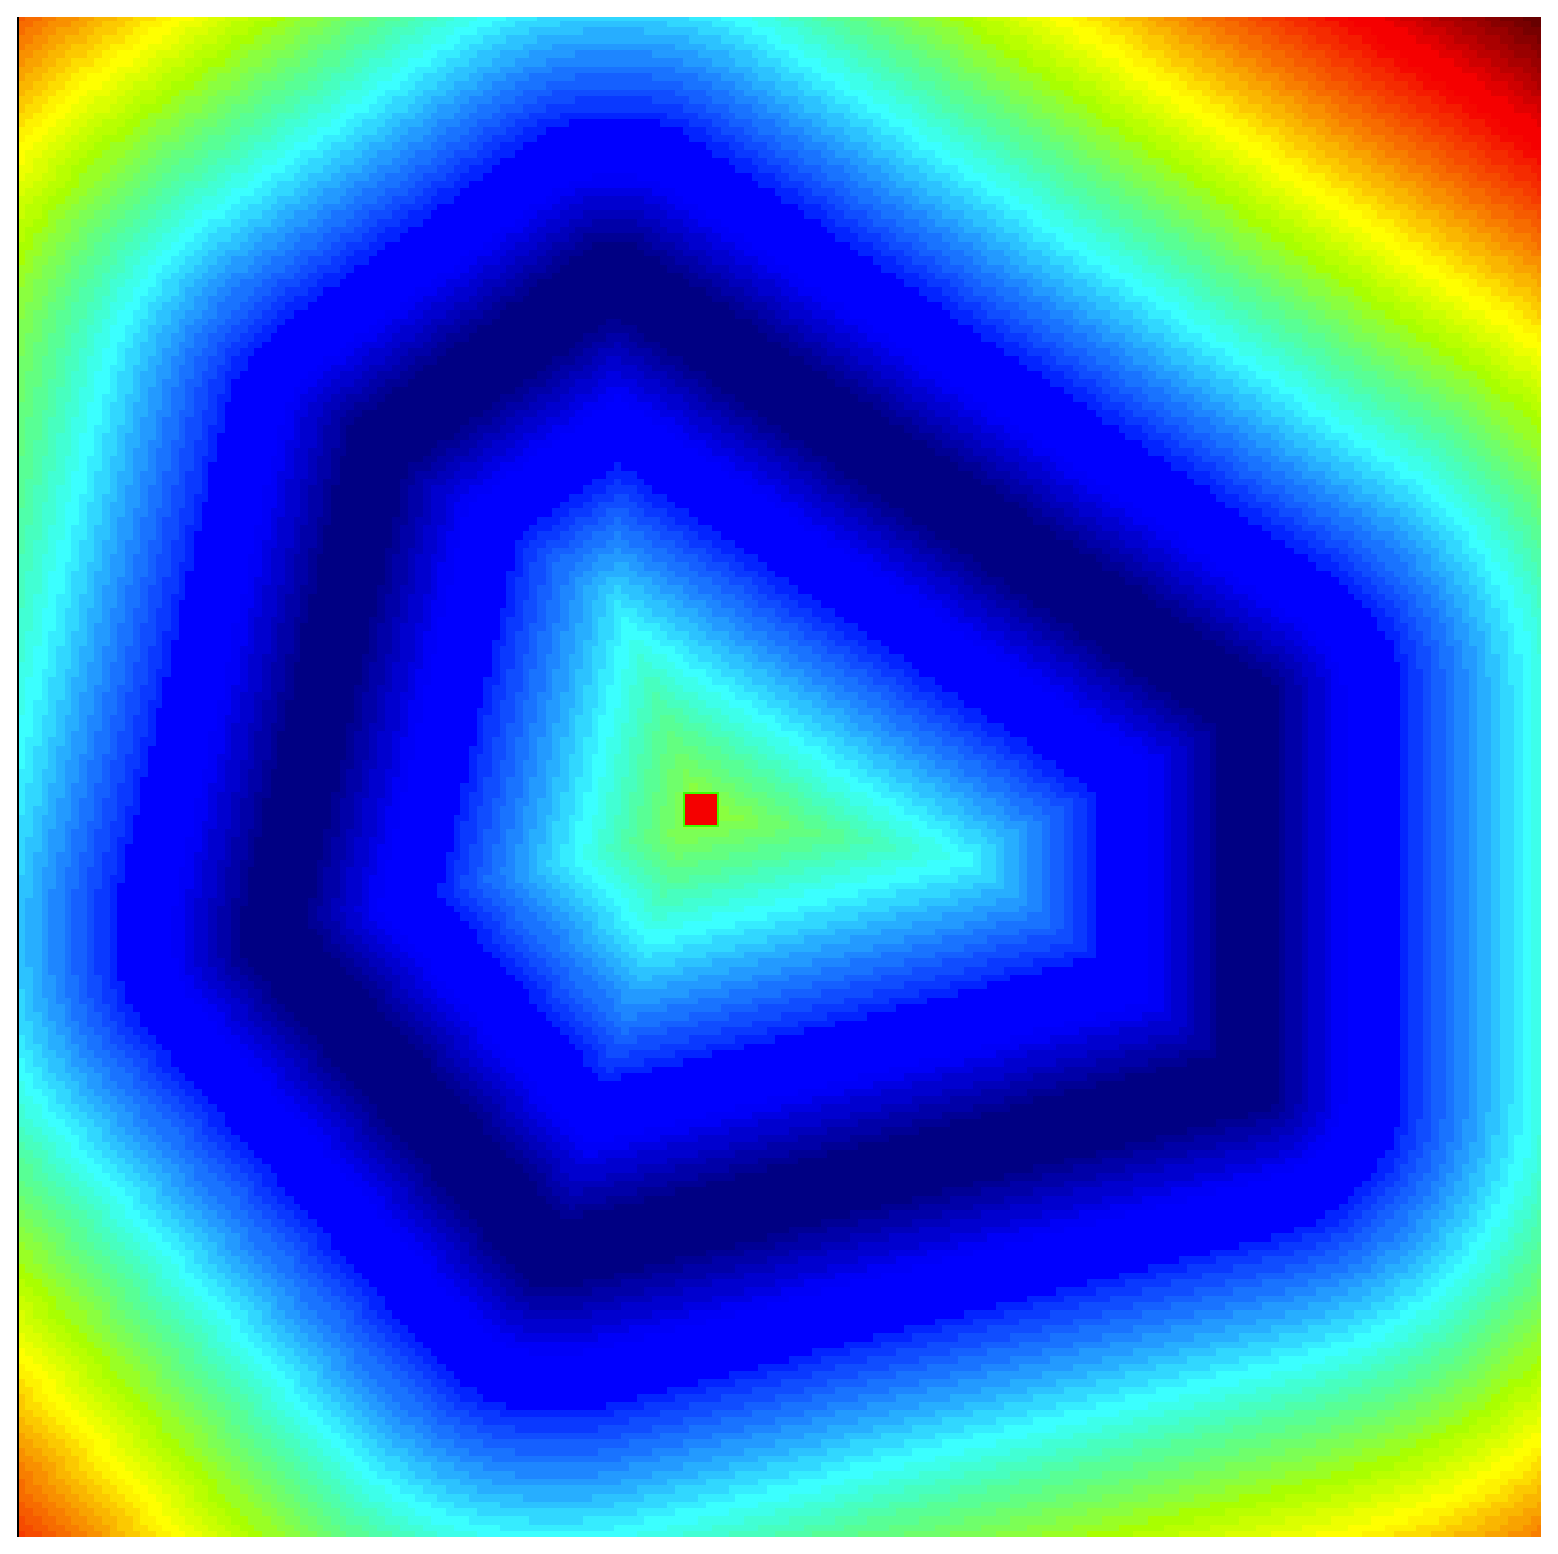
\includegraphics[width=0.33\textwidth, height=0.33\textwidth]{pictures/theoryCompleteCenter}\label{fig:theoryCompleteCenter}}\\
%
\subfloat[][]{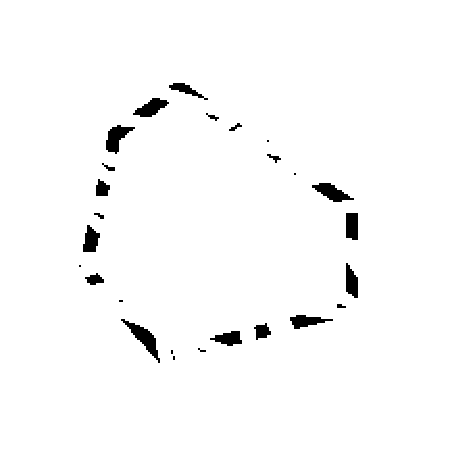
\includegraphics[width=0.33\textwidth, height=0.33\textwidth]{pictures/theoryIncomplete}\label{fig:theoryIncomplete}}
\subfloat[][]{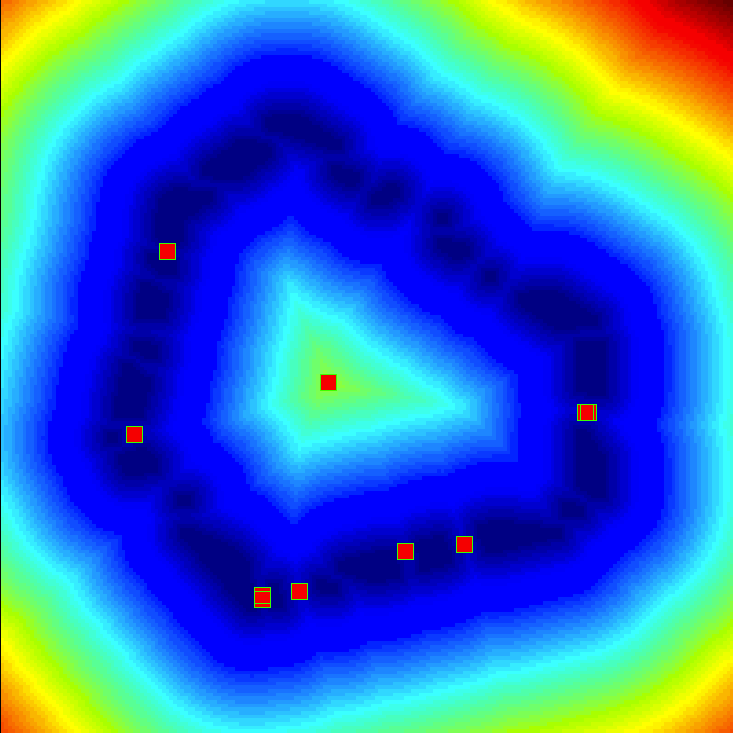
\includegraphics[width=0.33\textwidth, height=0.33\textwidth]{pictures/theoryIncompleteLocalMax}\label{fig:theoryIncompleteLocalMax}}
\subfloat[][]{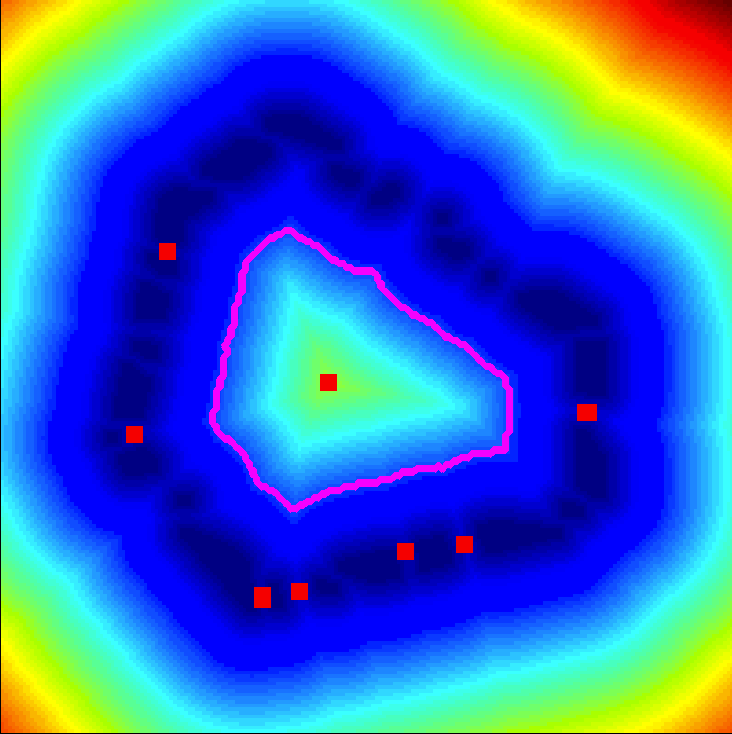
\includegraphics[width=0.33\textwidth, height=0.33\textwidth]{pictures/theoryIncompleteThreshold}\label{fig:theoryIncompleteThreshold}}\\
%
\subfloat[][]{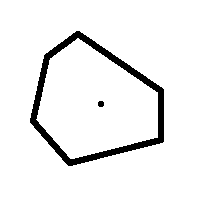
\includegraphics[width=0.33\textwidth, height=0.33\textwidth]{pictures/theoryNoise}\label{fig:theoryNoise}}
\subfloat[][]{\includegraphics[width=0.33\textwidth, height=0.33\textwidth]{pictures/theoryNoiseLocalMax}\label{fig:theoryNoiseLocalMax}}
\subfloat[][]{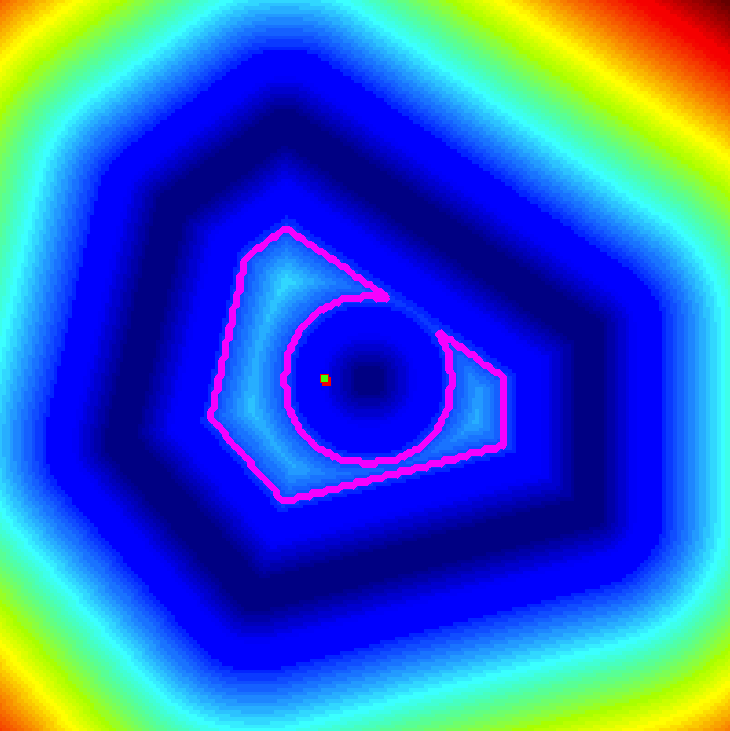
\includegraphics[width=0.33\textwidth, height=0.33\textwidth]{pictures/theoryNoiseCentroid}\label{fig:theoryNoiseCentroid}}
%
\caption{%
\subref{fig:theoryComplete}: complete synthetic cell membrane;
\subref{fig:theoryCompleteDistance}: distance map from~\subref{fig:theoryComplete};
\subref{fig:theoryCompleteCenter}: local maximum red square represents the local maxima of~\subref{fig:theoryCompleteDistance}.\\
%
\subref{fig:theoryIncomplete}:
 incomplete synthetic cell membrane;
\subref{fig:theoryIncompleteLocalMax}:
 distance map from~\subref{fig:theoryIncompleteLocalMax},
 the red squares are the local maximas;
\subref{fig:theoryIncompleteThreshold}: 
 thresold of~\subref{fig:theoryIncompleteLocalMax} 
 at 20pixels, represented by the magenta contour (approximation of the voronoi cell).
 Note that the only local maxima present in the
 thresholded area is the \emph{cell site}.\\
%
\subref{fig:theoryNoise}:
 noisy synthetic cell membrane;
\subref{fig:theoryNoiseLocalMax}:
 distance map from~\subref{fig:theoryNoise},
 the red squares are the local maximas;
\subref{fig:theoryNoiseCentroid}:
 threshold of~\subref{fig:theoryNoiseLocalMax} at 20pixels,
 represented by the magenta contour.
 Note that the centroid of the thresholded region (green square)
 is very close to the \emph{cell site} (red square).%
}
  \label{fig:incompleteMembraneSynthetic}
\end{figure}



\begin{figure}[htb]
  \centering
%
\subfloat[][]{\includegraphics[width=0.3\textwidth, height=0.3\textwidth]%
{pictures/propReconstructedMembrane}\label{fig:propReconstructedMembrane}}\hspace{3pt}
%
\subfloat[][]{\includegraphics[width=0.3\textwidth, height=0.3\textwidth]%
{pictures/propThresholdedReconstructed}\label{fig:propThresholdedReconstructed}}\hspace{3pt}
%
\subfloat[][]{\includegraphics[width=0.3\textwidth, height=0.3\textwidth]%
{pictures/propDistance}\label{fig:propDistance}}\\
%
%
%
%
%
%
\subfloat[][]{\includegraphics[width=0.3\textwidth, height=0.3\textwidth]%
{pictures/propNucleiMask}\label{fig:propNucleiMask}}\hspace{3pt}
%
\subfloat[][]{\includegraphics[width=0.3\textwidth, height=0.3\textwidth]%
{pictures/propDistThresh}\label{fig:propDistThresh}}\hspace{3pt}
%
\subfloat[][]{\includegraphics[width=0.3\textwidth, height=0.3\textwidth]%
{pictures/propDistThreshMask}\label{fig:propDistThreshMask}}\\
%
\subfloat[][]{\includegraphics[width=0.3\textwidth, height=0.3\textwidth]%
{pictures/propThresholdedDistanceMap}\label{fig:propThresholdedDistanceMap}}\hspace{3pt}
%
\subfloat[][]{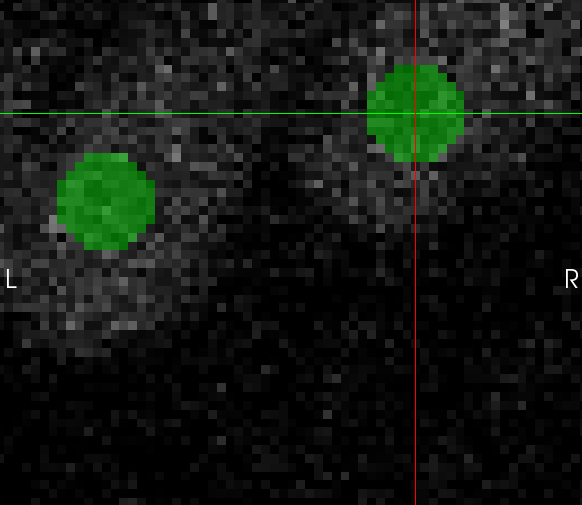
\includegraphics[width=0.3\textwidth, height=0.3\textwidth]{pictures/propCentroids}\label{fig:propCentroids}}\\
%
\caption{\\%
Figures \subref{fig:propReconstructedMembrane}, \subref{fig:propThresholdedReconstructed}, \subref{fig:propDistance}: Distance map creation from the reconstructed membrane data.\\
\subref{fig:propReconstructedMembrane}: Reconstructed membrane with\cite{kishoreMembrane};
\subref{fig:propThresholdedReconstructed}: Binary image of the membrane;
\subref{fig:propDistance}: Distance map created from the incomplete membrane data (red values are higher, and dark values are lower).\\
\\
%
%
Figures \subref{fig:propNucleiMask}, \subref{fig:propDistThresh}, \subref{fig:propDistThreshMask}, \subref{fig:propThresholdedDistanceMap}, \subref{fig:propCentroids}: Localisation of the \emph{sites} from the threshoded distance map and the thresholded nuclei channels:\\
\subref{fig:propNucleiMask}: Nuclei mask used for masking the approximate VRs;
\subref{fig:propDistThresh}: Thresholded distance map of the membrane : approximate VRs;
\subref{fig:propDistThreshMask}: Masked approximate VRs. Their \emph{centroid} is to the \emph{cell site}.
\subref{fig:propThresholdedDistanceMap}: Close up of two approximate VRs masked with the thresholded nuclei;
\subref{fig:propCentroids}: Nuclei detection (in green) corresponding to the \emph{centroids} of the masked approximate VRs of figure~\subref{fig:propThresholdedDistanceMap}.%
}
  \label{fig:propIllustr}
\end{figure}




\subsection{Difficulties and solutions}
\label{sect:difficultiesTheory}

\subsubsection{Profusion of local maximas}

As the membrane is a convex polygon, we should have only one local maxima per VR, 
and from that, determining the VS should be easy, but,
the lack of information on the membrane channel creates local maxima in the holes location (as illustrated figure~\ref{fig:theoryIncompleteLocalMax}).
If the holes in the membrane are much smaller than the cell's radius,
those unwanted local maximas will have much smaller value than the one in the middle of the cell,
because they will be close to the hole's boundary.
We use a simple threshold on the distance map to invalidate smaller local maximas, and keep the high values of the distance map (see figure~\ref{fig:theoryIncompleteThreshold}), this gives us a region inside the VR, that we name "approximate VR".
This region is inside the VR, and can be considered as an erosion of it. 

Another reason for having several local maximas, is noise in the membrane channel (as illustrated figure~\ref{fig:theoryNoise}).
If a point far from the boundary of the cell is considered as membrane, the distances will be computed from this point, leading to two local maximas in one cell, of lower value (see figure~\ref{fig:theoryNoiseLocalMax}). This modifies the shape of the approximate VR, and the position of its center of mass.
If the noise is restricted to few points in the membrane, then we are able to recover the VS by computing the center of mass of the thresholded distance map (see figure~\ref{fig:theoryNoise}, \subref{fig:theoryNoiseLocalMax}, \subref{fig:theoryNoiseCentroid}).

\subsubsection{Shape of cell membranes}

In order to find an eroded approximation of the Voronoi cell, we use a simple thresholding on the distance map generated from the membrane.
Then, we locate the centroid of this region, but it happens that cells are not convex polygons, and in this case, the centroid can be outside the membrane (especially in bean shaped cells).
In order to keep the centroid inside the cell boundaries, we mask the Voronoi approximation, by the binarized nuclei channel.
Thus, our regions are restricted to parts of the image where a nuclei is present, and the centroid of the masked approximate Voronoi cell is located inside the nuclei.

\subsubsection{Membrane reconstruction}

As the membrane information is very poor, we use, a reconstruction method designed by Dr Kishore Mosaliganti {\etal}~\cite{kishoreMembrane}. This method is inspired by~\cite{tasdizen2005enhancement}, who presents a method for cell boundaries enhancement in 2D.
These methods are inspired by vessel enhancement techniques~\cite{frangi1998multiscale, manniesing2006vessel}.
The vessel enhancement algorithms' assumption is that vessel are constituted by succession of cylinders. Kishore's assumption is that membrane is constituted by plans.
Kishore's algorithm diffuses intensities along planar structures, instead of cylinders.

This method provides a very good denoising, but big holes in the membrane channel are still presents. In order to fill those holes and get a reconstructed membrane, Kishore uses a tensor voting reconstruction method~\cite{tensorvoting}.



%%%%%%%%%%%%%%%%%%%%%%%%%%%%%%%%%%%%%%%%%%%%%%%%%%%%%%%%%%%%%%%%%%%%%%%%%%%%%%%
%%%%%%%%%%%%%%%%%%%%%%%%%%%%%%%%%%%%%%%%%%%%%%%%%%%%%%%%%%%%%%%%%%%%%%%%%%%%%%%
%%%%%%%%%%%%%%%%%%%%%%%%%%%%%%%%%%%%%%%%%%%%%%%%%%%%%%%%%%%%%%%%%%%%%%%%%%%%%%%


\section*{Conclusion}

We present here a new method for detecting cell nuclei in noisy and incomplete 2 photon/confocal 3D datasets.
This method uses a simple assumption, and we proved that it is robust to loss of continuity in the membrane channel, and noise.
We described the theory, and explained the methodology, we will evaluate this method against existing algorithms to finally conclude about our contribution.



